\chapter{Bounce Event Detection}
\label{ch:bounce}

This chapter applies the protocol of Chapter~\ref{ch:methodology} to the third
perception sub-task: deciding at which frames the ball bounces on the court, given
the trajectory it traces through a rally. Ball tracking locates the ball in each
frame (Chapter~\ref{ch:ball}) and court detection registers the playing surface
(Chapter~\ref{ch:court}); bounce detection differs from both in that it consumes
the output of the tracker rather than the raw image. Its input is a
one-dimensional time series of ball positions, and its task is to mark the moment
of ground contact within it. The sub-task runs on the TrackNet tennis dataset of
Section~\ref{sec:meth-tracknet}, under the bounce-specific split of
Section~\ref{sec:meth-splits-tracknet} that holds out match game7 as the test set,
and it is scored by the event-detection metrics of
Section~\ref{sec:meth-metrics-event}. Two learned models are trained for that: a
gradient-boosted per-frame classifier and a small temporal convolutional network,
compared on one shared trajectory pipeline. The chapter answers the third
research question (RQ3) of Section~\ref{sec:intro-objectives}: how the two models
compare in accuracy, and what each costs in engineering effort.

\section{Task Formulation}
\label{sec:bounce-task}

A bounce is the frame at which the ball hits the court, recorded in the dataset
as status~2 in the annotation schema of Section~\ref{sec:meth-tracknet-schema}.
The task is posed as event detection in time rather than as per-frame
classification, for the reason set out in Section~\ref{sec:meth-metrics-event}:
bounce frames make up only 2.6\,\% of the data
(Table~\ref{tab:tracknet-labels}), so a per-frame accuracy would be dominated by
the negative class.

The problem is that the signature of a bounce is not unique to bounces. That is what
makes the task hard and rules out a simple solution. A racket hit, status~1 in the
same schema and almost as frequent as a bounce (516 against 523 events across the
dataset, Table~\ref{tab:tracknet-labels}).
Figure~\ref{fig:bounce-trajectory-motivation} shows both effects within a single
rally. Separating a bounce from a hit depends on the finer shape of the
trajectory around the reversal, which neither the reversal nor the ball's position
reveals on its own. That shape is the distinction the two learned models are
trained to understand.

\begin{figure}[t]
  \centering
  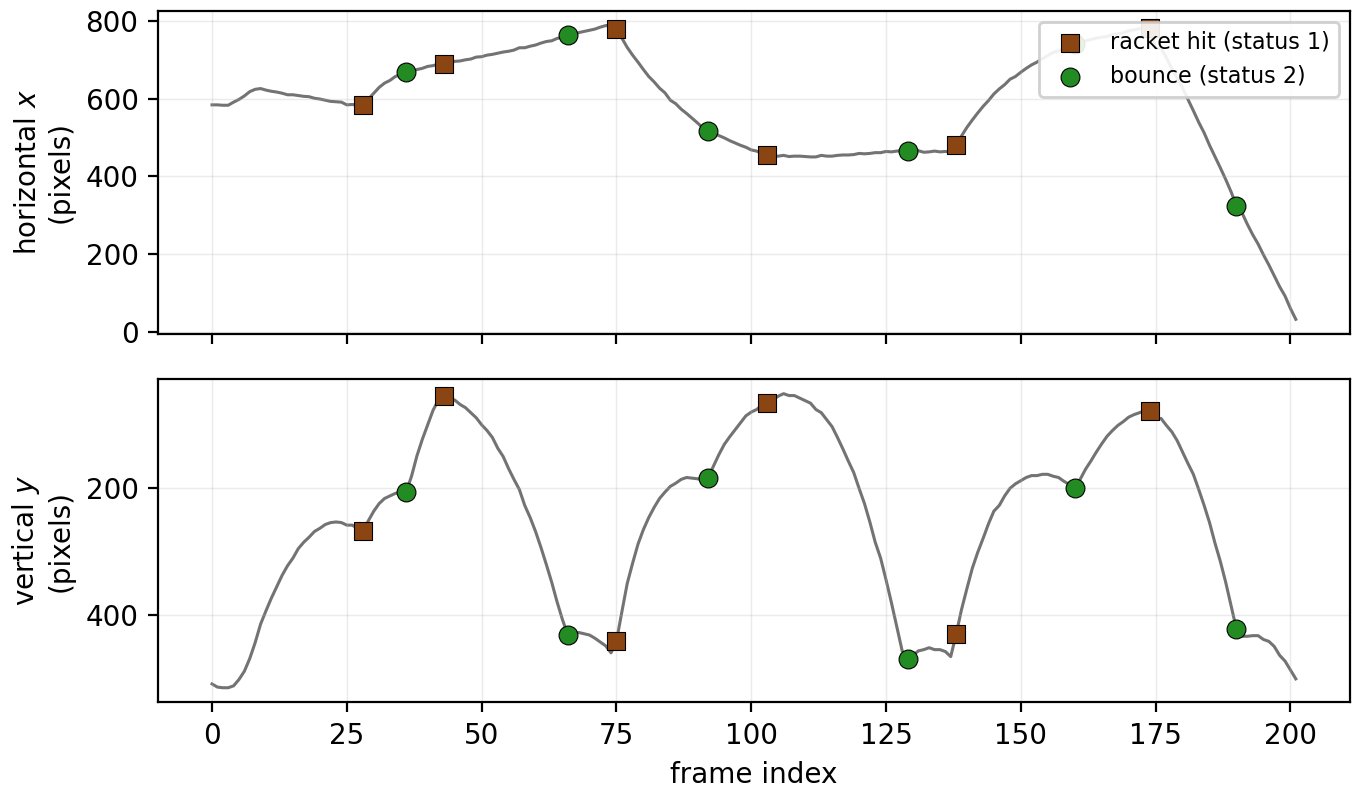
\includegraphics[width=\linewidth]{img/bounce_trajectory_motivation.png}
  \caption{The bounce signature in the ball-coordinate time series, for one rally
    of the game7 test split with six bounces and six hits. The horizontal ($x$)
    and vertical ($y$) image coordinates are plotted against the frame index; the
    vertical axis is inverted so the court lies toward the bottom of the panel.
    Bounce frames (status~2) are marked in green and racket hits (status~1) in
    brown.} 
  \label{fig:bounce-trajectory-motivation}
\end{figure}

One scope limitation must be stated at the beginning. The trajectory fed to both
models in this chapter is built from the ground-truth ball coordinates recorded
in the dataset, not from the output of the ball tracker of Chapter~\ref{ch:ball}.
The reported scores are therefore an upper bound on the performance of a deployed
system, in which the trajectory would carry the localisation error of the tracker,
which is largest on exactly the occluded and near-ground frames where a bounce
occurs. This decision isolates the bounce-detection question from the
ball-tracking question, so that the two models are compared on the same
clean signal.

\section{Trajectory Processing and Features}
\label{sec:bounce-features}

Both models share a single trajectory pipeline, so that the comparison keeps the same preprocessing, learning target,
decoding, and metrics fixed. The pipeline operates strictly within each clip,
so that no feature, window, or smoothing operation ever crosses a clip boundary
where the ball identity and the time base are discontinuous.

The pipeline begins by cleaning the raw trajectory, the sequence of annotated ball
positions in a clip, sorted by frame index. Frames carrying the $(-1, -1)$ missing-ball sentinel of
Section~\ref{sec:meth-tracknet}, whether from an invisible ball or a blank
annotation, are converted to gaps. Short internal gaps of at most four frames are
filled by linear interpolation, on the assumption that the ball follows a smooth
path over so short an interval. Longer gaps and gaps at the start
or end of a clip are left unfilled and are masked out of both the learning target
and the loss, so that the detector is never trained or scored on a stretch of
trajectory that does not exist.

The cleaned positions are then differentiated to recover the velocity and
acceleration that carry the bounce signature. On each consecutive run of valid frames of length
at least seven, a Savitzky-Golay smoothing-differentiation filter with a
seven-frame window and a quadratic polynomial estimates the first and second
derivatives, which suppresses the per-frame jitter that a naive finite difference
would amplify; shorter runs fall back to central differences. This yields the
horizontal and vertical velocity and acceleration at every valid frame.
Figure~\ref{fig:savgol-vs-finite-difference} contrasts the two estimates on a
single rally: the finite difference is visibly noisier, most of all in the
acceleration, whereas the Savitzky-Golay filter preserves the reversal at each
bounce while suppressing the jitter.

\begin{figure}[t]
  \centering
  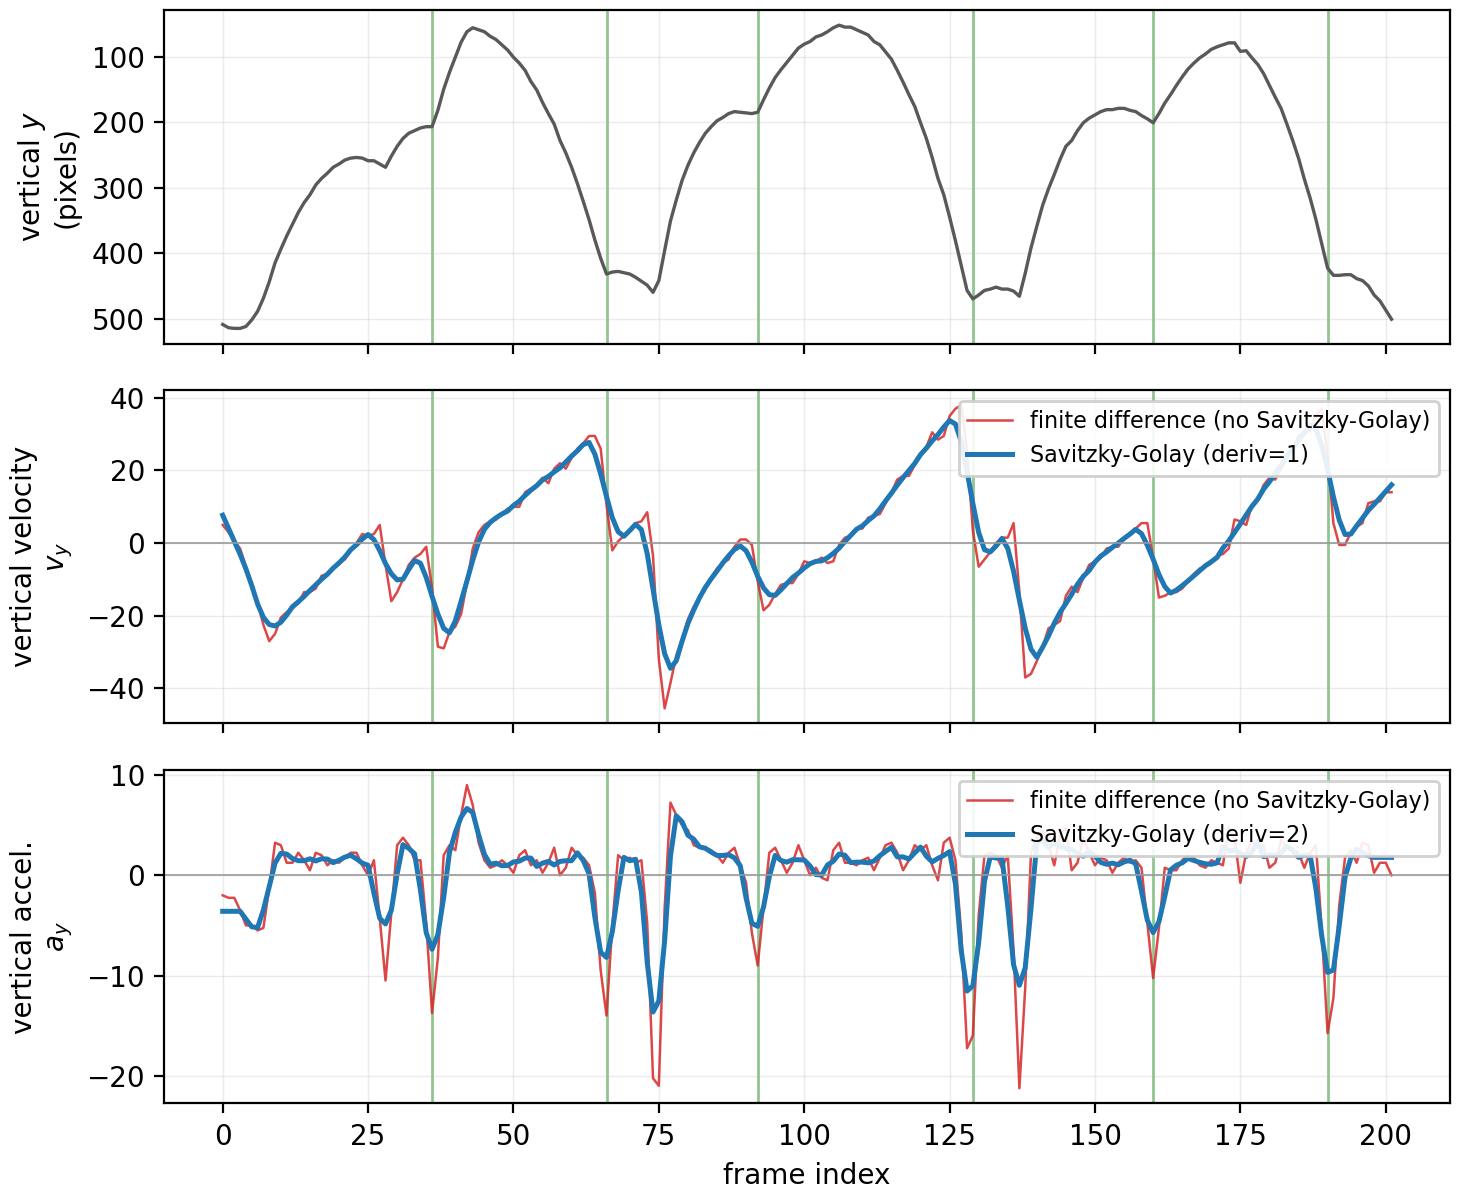
\includegraphics[width=\linewidth]{img/savgol_vs_finite_difference.png}
  \caption{Velocity and acceleration recovered from the vertical ball trajectory
    of one rally, comparing a naive finite difference (red) with the
    Savitzky-Golay smoothing-differentiation filter (blue). Top: the vertical image
    coordinate $y$ against the frame index, with bounce frames marked in green.
    Middle: the first derivative $v_y$. Bottom: the second derivative $a_y$. The
    finite difference amplifies the per-frame jitter in the tracked positions, most
    severely in the acceleration, while the Savitzky-Golay estimate keeps the
    reversal at each bounce and rejects the noise.}
  \label{fig:savgol-vs-finite-difference}
\end{figure}

From this cleaned and differentiated trajectory, two feature representations are
derived, one for each kind of model. For the gradient-boosted model, which sees one frame at a
time, each frame is described by a seventy-one-dimensional vector: eleven base
quantities, namely the normalised position, the velocity and acceleration
components, the speed and acceleration magnitude, the change in heading, the
visibility, and the interpolation flag, together with sixty lag features that
encode the local shape of the trajectory. The lag features compare each frame with
its neighbours up to ten frames away in both directions, as signed vertical
differences, absolute horizontal differences, and, most importantly, the
scale-invariant ratios of the forward to the backward difference. These ratios are
the principal discriminative feature: in free flight the trajectory is locally
monotonic and the ratio of forward to backward motion is close to $-1$, whereas at
a bounce the motion reverses and the ratio flips towards $+1$. For the temporal convolutional network, which sees
a window of frames at once and can learn such lag structure internally, each frame
is described by only seven channels: the normalised position, the velocity and
acceleration components, and the visibility.

The learning target is common to both learned models and is a soft one. Rather
than a single positive frame per bounce, which would make an off-by-one prediction
count as a complete miss and would offer almost no gradient on the scarce positive
class, the target is a Gaussian bump in time of unit peak and a standard deviation
of $1.5$ frames, centred on each bounce frame. Hits and ordinary in-flight frames
carry a target of zero, so that the soft label rewards a prediction near a true
bounce in proportion to its temporal closeness while still treating hits as
negatives.

\section{Models}
\label{sec:bounce-models}

Two models are compared, each mapping a clip's trajectory to a per-frame bounce
score in $[0, 1]$ that the shared decoder of Section~\ref{sec:bounce-decode} turns
into discrete events. Both are learned models that draw the bounce-against-hit
distinction the task demands, but they differ in how much of the trajectory shape
is supplied to them and how much they must learn. The gradient-boosted classifier
is handed an explicit per-frame description of the local trajectory shape, while
the temporal convolutional network is given only the raw per-frame channels and
must learn that shape for itself. This contrast, between an engineered-feature model
and an end-to-end temporal one, is the comparison RQ3 needs.
Table~\ref{tab:bounce-models} summarises them.

\begin{table}[t]
  \centering
  \small
  \setlength{\tabcolsep}{5pt}
  \caption{The two bounce-detection models. The input column distinguishes
    the per-frame model from the windowed one; the trained-parameters column
    counts only learned weights, excluding the single decode threshold that both
    calibrate on the validation split.}
  \label{tab:bounce-models}
  \begin{tabular}{@{}l p{3.0cm} p{3.1cm} l@{}}
    \toprule
    Approach & Input per prediction & Discriminative mechanism & Trained params \\
    \midrule
    XGBoost & one frame, 71 features & boosted regression trees & 515 trees ($\le\!10^3$) \\
    TCN & 64-frame window, 7 channels & dilated temporal convolutions & 10{,}433 weights \\
    \bottomrule
  \end{tabular}
\end{table}


The gradient-boosted model is an ensemble of regression trees, in the gradient
boosting framework of Friedman~\cite{friedman2001gbm}, that maps the
seventy-one-dimensional per-frame feature vector of Section~\ref{sec:bounce-features}
to the soft bounce target. The implementation is XGBoost~\cite{chen2016xgboost}, gradient-boosting model that fits each new tree to the second-order
expansion of a regularised objective and searches for its splits over histogram bins
of the features, so that training over the full per-frame table is both efficient and
resistant to overfitting. It is trained to minimise the squared error against the
soft target, with the frames near a bounce up-weighted so that the scarce positive
region is not drowned out by the negative class, for up to a thousand boosting
iterations with early stopping on a held-out validation split.


The temporal convolutional network processes a window of sixty-four consecutive
frames of the seven-channel representation and emits a bounce logit for every frame
in the window, in the style of temporal convolutional models for sequence
labelling~\cite{lea2017tcn,bai2018tcn}. It is a small stack of four residual
blocks of dilated one-dimensional convolutions, with the dilation doubling from one
block to the next so that the receptive field grows exponentially and a single
output frame can attend to its wider temporal neighbourhood, the same mechanism
that lets dilated convolutions model long-range structure in sequence
data~\cite{vandenoord2016wavenet}. The network is kept deliberately small, only
10{,}433 weights in the configuration used here, because the positive class is
scarce and a larger model would overfit the few hundred training bounces. It is
trained with the
Adam optimiser~\cite{kingma2015adam} against the soft target under a masked focal
binary cross-entropy loss that down-weights the easy negative frames and up-weights
the rare positives, with the loss masked out on the invalid frames identified by
the cleaning step. At inference the network is run over overlapping windows whose
predictions are averaged back into a single per-frame score for the clip. Unlike
the gradient-boosted model it learns its own temporal features from the raw
channels, at the cost of a training loop, and a hardware accelerator to train on.
\section{Decoding and Event Matching}
\label{sec:bounce-decode}

To keep the comparison fair, the per-frame scores of both models pass through
one shared decoder, so that any difference in the reported
events is a difference between the scores and not between the post-processing. The
decoder locates the peaks of the score signal that exceed the model's threshold, subject to a minimum spacing of five frames between successive peaks so
that a single bounce is not reported twice, and treats each surviving peak as one
predicted bounce event; frames masked invalid by the cleaning step are excluded
from the search. The predicted events are then matched to the ground-truth bounce
frames by the greedy one-to-one assignment within $\pm k$ frames defined in
Section~\ref{sec:meth-metrics-event}, closest pair first, from which the true
positives, false positives, and false negatives, and hence the event precision,
recall, and $F_1$ at tolerance $k$, follow. The default tolerance is $k = 3$
frames, and a sweep over $k \in \{0, 1, 2, 3, 5, 7\}$ reports how the score
tightens or relaxes with the timing requirement.

\section{Results}
\label{sec:bounce-results}

The models were evaluated on the game7 test split, a single held-out match
of 1\,881 frames in nine clips containing 50 bounce events
(Table~\ref{tab:splits}). Each model's decode threshold was the value calibrated on
the validation split. Table~\ref{tab:bounce-results} reports the event metrics at
the default tolerance together with the average precision and the event counts, for
the four boosting libraries and the temporal network, and
Figure~\ref{fig:bounce-comparison} plots the tolerance sweep and the
precision-recall curves for the selected XGBoost model against the network.

\begin{table}[t]
  \centering
  \footnotesize
  \setlength{\tabcolsep}{4pt}
  \caption{Bounce-detection results on the game7 test split (50 bounce events), at
    the default tolerance $k = 3$ frames. $P$, $R$, and $F_1$ are the event
    precision, recall, and $F_1$ at that tolerance; AP is the average precision over
    the threshold sweep; TP, FP, and FN are the event counts. Bold marks the best
    value in each column.}
  \label{tab:bounce-results}
  \begin{tabular}{l r r r r r r r r}
    \toprule
    Model & $F_1$ & $P$ & $R$ & AP & TP & FP & FN & FPS \\
    \midrule
    \textbf{XGBoost} & 0.948 & \textbf{0.979} & 0.920 & 0.930 & 46 & \textbf{1} & 4 & \textbf{36{,}045} \\
    HistGBM          & \textbf{0.951} & 0.925 & \textbf{0.980} & 0.874 & 49 & 4 & \textbf{1} & 23{,}211 \\
    LightGBM         & \textbf{0.951} & 0.925 & \textbf{0.980} & 0.866 & 49 & 4 & \textbf{1} & 30{,}610 \\
    CatBoost         & \textbf{0.951} & 0.925 & \textbf{0.980} & 0.771 & 49 & 4 & \textbf{1} & 34{,}910 \\
    \midrule
    TCN              & 0.925 & 0.875 & \textbf{0.980} & \textbf{0.972} & 49 & 7 & \textbf{1} & 1{,}788 \\
    \bottomrule
  \end{tabular}
\end{table}

\begin{figure}[t]
  \centering
  \begin{subfigure}{0.49\textwidth}
    \centering
    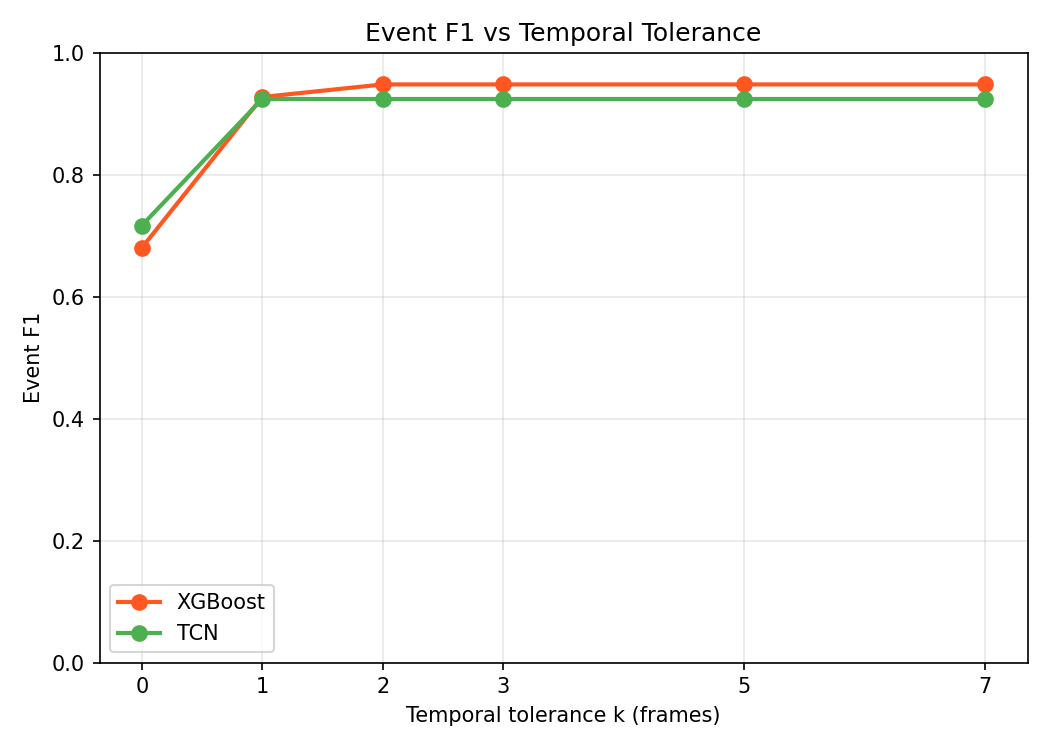
\includegraphics[width=\linewidth]{img/bounce_f1_vs_tolerance.png}
    \caption{$F_1$ across the tolerance sweep.}
    \label{fig:bounce-f1k}
  \end{subfigure}\hfill
  \begin{subfigure}{0.49\textwidth}
    \centering
    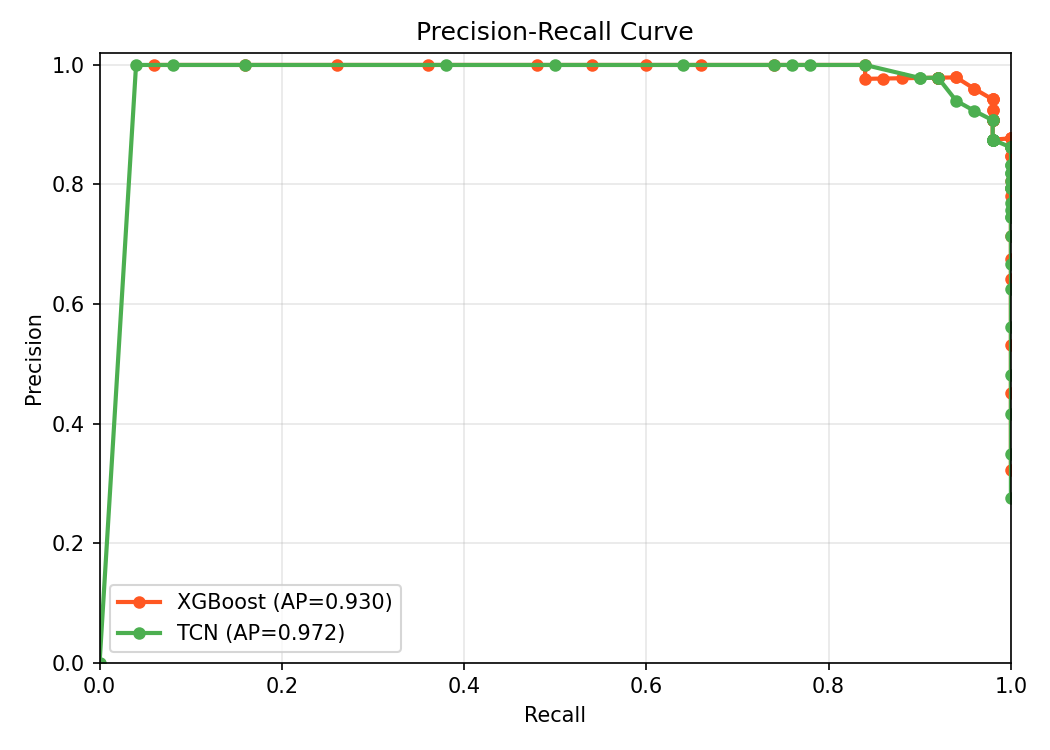
\includegraphics[width=\linewidth]{img/bounce_pr_curve.png}
    \caption{Precision-recall curves.}
    \label{fig:bounce-pr}
  \end{subfigure}
  \caption{Bounce-detection comparison on the game7 test split, for the selected
    XGBoost model against the temporal network. (a)~Event $F_1$ as the matching
    tolerance $k$ widens from $0$ (exact frame) to $7$ frames. At the exact frame the
    temporal network achieves the higher $F_1$ (0.717 against XGBoost's 0.680), but
    from $k = 2$ onward XGBoost leads, and both models plateau by $k = 2$. (b)~The
    precision-recall curves traced by sweeping the decode threshold, whose areas are
    the average precisions of Table~\ref{tab:bounce-results}: the temporal network
    encloses the larger area (AP 0.972 against 0.930).}
  \label{fig:bounce-comparison}
\end{figure}

The four boosting libraries are, for practical purposes, the same model. Their
event $F_1$ spans 0.948 to 0.951, and three of them, the histogram regressor of
scikit-learn, LightGBM, and CatBoost, return the identical confusion of 49 recovered
bounces, four false positives, and one miss; only XGBoost departs from it, and only
at its operating point. What separates the four is not their $F_1$ but the quality of
their score ranking, which the average precision measures: XGBoost reaches 0.930,
well clear of the 0.874, 0.866, and 0.771 of the histogram model, LightGBM, and
CatBoost, so it is the least sensitive of the four to where the decode threshold is
placed. On that robustness, together with its operating-point precision, XGBoost is
the gradient-boosted model carried forward, and the comparison that follows is
between it and the temporal network.

Against the network the two models solve the task about equally well but trade their
errors differently. At the default tolerance XGBoost attains the higher event $F_1$,
0.948 against 0.925,and it raises a single
false positive across the whole test match, for a precision of 0.979, where the
network raises seven, for 0.875. It pays for that caution in recall, recovering 46 of
the 50 bounces against the network's 49, so the network is the more complete detector
and XGBoost the more conservative one. The contrast is the familiar one between a
precision-favouring and a recall-favouring operating point rather than a gap in
capability.

The two lead on different measures, and the swap is informative rather than
contradictory. On the average precision, which integrates over all decode thresholds
and so measures the quality of the score ranking independently of any one operating
point, the temporal network is ahead, at 0.972 against 0.930. On the exact-frame
tolerance $k = 0$ in Figure~\ref{fig:bounce-f1k} it is again ahead, at 0.717 against
0.680, which says it places the peak on the true bounce frame more often; from
$k = 2$ onward, XGBoost takes the lead on
$F_1$ and both plateau. As Section~\ref{sec:meth-metrics-event} cautions, the average
precision and the $F_1$ at a tolerance are different quantities at different operating
points, and on a test set of only fifty events a few false positives or a few missed
bounces are enough to separate two otherwise closely matched models. The fair summary
is that the temporal network has the better score ranking, exact-frame timing, and
recall, while XGBoost is the more precise at the deployed threshold.

These results answer RQ3. Both models solve the timing problem well, each
exceeding an $F_1$ of 0.92 and almost never mistaking a hit for a bounce, which
confirms that learning the trajectory shape succeeds where reading the reversal
alone could not. Between the two the difference is small and direction-dependent,
the temporal network holding the better average precision, exact-frame timing, and
recall, and XGBoost the better $F_1$ and precision. The
engineering costs that separate them, and the consequences of the
ground-truth-trajectory ceiling, are the subject of the analysis below and inform
the model carried into the integrated system of Chapter~\ref{ch:integrated}.

\section{Analysis}
\label{sec:bounce-analysis}

The finding is that the bounce signature is learnable but not reducible to a
simple rule. The cues that mark a bounce, the local maximum of the vertical
position, the velocity sign flip, and the acceleration spike, are genuinely present
at every bounce, but they are equally present at racket hits and at the apex of
every flight, so a detector that thresholds those cues directly cannot resolve the
ambiguity, as Section~\ref{sec:bounce-task} argued from the trajectory itself. Both
learned models succeed on exactly this hit-against-bounce distinction, because they
exploit the finer differences in trajectory shape around the two kinds of event
rather than responding to the reversal alone, and their near-perfect separation of
the two classes confirms that the discriminative information lies in that shape.
This parallels the finding of Chapter~\ref{ch:ball} that a learned localiser
outperforms a geometric one.

Two further caveats qualify the numbers. First, the test set is a single held-out
match with only fifty bounce events, in keeping with the scope noted in
Section~\ref{sec:intro-scope}, so each event is worth two points of recall and a
difference of a few false positives moves the $F_1$ by several points; the gap
between the two learned models in particular should not be over-read, and the
per-game breakdown collapses to this one match. Second, the location of each bounce
in court metres, which the integrated system uses for its line call, is not scored
anywhere in this chapter, because the TrackNet dataset carries no court-keypoint
ground truth and so no in-or-out label against which a projected bounce position
could be checked; the court projection of a detected bounce is therefore a
qualitative capability of the integrated system, taken up in
Chapter~\ref{ch:integrated}, and not a measured result.

In summary, the bounce sub-task answers RQ3 as follows. Separating bounces from the
racket hits that share their kinematic signature calls for a model of the
trajectory shape, not a rule on the reversal. A gradient-boosted model and a small
temporal convolutional network draw that distinction about equally well, and XGBoost, the strongest of the four boosting libraries
tried, is preferred for the integrated system on the strength of its operating-point
precision and its markedly simpler deployment.